\section{Systematic uncertainties}
%%%%%%%%%%%%%%%%%%%%%%%%%%%%%%%%%%%%%%%%%%%%%%%%%%%%%%%%%%%%%%%%%%%%%%
\label{sec:Systematics}

Systematic uncertainties play an important role in this analysis where
no strong mass peak is expected due to the presence of undetected
neutrinos in the final state.  One of the most important sources of
systematic uncertainty is the normalization of the backgrounds that
are estimated on data control samples whenever is possible.

A summary of the main sources of systematic uncertainty and the corresponding estimate is reported in Table~\ref{tab:Systematics}. A detailed description of each source of systematic uncertainty is discussed in the following sections.

\begin{table}[h]
\small{
  \begin{center}
  \caption{Main sources of systematic uncertainties and their estimate. The
  first category reports the uncertainties in the normalization of background
  contributions. The experimental and theoretical uncertainties refer to the
  effect on signal yields. A range is specified if the uncertainty varies
  across the $\pth$ bins.}
  \label{tab:Systematics}
  \begin{tabular}{cc}
  \hline\hline
  \multicolumn{2}{c} {\bf{Uncertainties in backgrounds contributions}} \\
  \hline
  Source  & Uncertainty \\
  \hline
  $\rm{t\bar{t}}$, tW      & 20--50$\%$ \\
  W+ jets              & $40\%$ \\
  WZ, ZZ              & $4\%$ \\
  W$\gamma^{(*)}$  & $30\%$ \\
  \hline\hline
  \multicolumn{2}{c} {\bf{Effect of the experimental uncertainties on the signal and background yields}}\\
  \hline
  Source & Uncertainty\\
  \hline
  Integrated luminosity        & $2.6\%$ \\
  Trigger efficiency           & 1--2$\%$\\
  Lepton reconstruction and identification & 3--4$\%$\\
  Lepton energy scale          & 2--4$\%$ \\
  \MET modelling          & $2\%$ \\
  Jet energy scale             & $10\%$ \\
  Pileup multiplicity          & $2\%$ \\
  b mistag modelling	       & $3\%$ \\	
  \hline\hline
  \multicolumn{2}{c}{\bf{Effect of the theoretical uncertainties on signal yield}}\\
  \hline
  Source & Uncertainty \\
  \hline
  b jet veto scale factor              & 1--2$\%$\\
  PDF                                  & $1\%$ \\
  WW background shape                  & $1\%$\\
  \hline
  \end{tabular}
  \end{center}
}
\end{table}


%-------------------------------------------------------------------------------
\subsection{Background normalization uncertainties}
%-------------------------------------------------------------------------------

The signal extraction is performed subtracting the estimated backgrounds to the event counts in data.
This uncertainty depends on the background: 
  \begin{itemize}
    \item {\bf\boldmath \ttbar and tW backgrounds:} 
      The efficiency on jets b-tagging is estimated using the Tag\&Probe technique in data
      and simulation control regions, as explained in \ref{sec:TagAndProbe}. 
      A per-jet scale factor, which takes into account the possibly different efficiency of the anti b-tagging selection in data and simulation, 
      is computed by means of the efficiency measured with the Tag\&Probe method.
%      \begin{equation}
%      w_{b-tag}^{n} = \left( \frac{1-\epsilon_{b-tag}^{DATA}}{1-\epsilon_{b-tag}^{MC}} \right)^n
%      \end{equation}
%      where $w_{b-tag}^{n}$ is the weight applied to events in the signal region with $n$ true 
%      b-jets and $\epsilon_{b-tag}^{DATA}$ and $\epsilon_{b-tag}^{MC}$ are the per-jet b-tagging efficiencies measured in data and MC respectively. 
      The Tag\&Probe method has been used also to measure the mistag rates in data and simulation, which are the probability to b-tag a jet that is not produced by the hadronization of a b quark.
%      The mistag scale factor $w_{mistag}^{n}$ is evaluated as:
%      \begin{equation}
%      w_{mistag}^{n} = \left( \frac{1-\epsilon_{mistag}^{DATA}}{1-\epsilon_{mistag}^{MC}} \right)^n
%      \end{equation}
      These factors are used to reweigh the Top MC samples as explained in \ref{sec:TTBackground}. The uncertainties provided by the Tag\&Probe fit are then propagated to the factor $\alpha$ that is used in the top data driven estimation \ref{sec:DD}.
      These uncertainties are embedded in a systematic error that affects the shape of the Top background in each \pth bin.
      
      Provided that the simulated samples include both \ttbar and tW processes, a systematic uncertainty related to the tW$/$\ttbar fraction has been included.
      In fact, a relative variation of the contribution of these two processes could modify the shape of the MC sample, and is thus included as a shape uncertainty affecting the top quark background shape in each \pth bin in a correlated way. 
      %The associated uncertainty ($\sim$30\%) is 
      %shared between the statistical of the control sample and the 
      %systematic one.
 
    \item {\bf\boldmath W+jets background:} It is estimated with data control
      sample as described in Sec.\ref{sec:wjetsbkg}. With 19.4\ifb at 8 \TeV,
      the uncertainty receives similar contributions from statistics
      and systematic error (mainly jet composition differences
      between the fake rate estimation sample and the application
      sample), the total error being about 40\%, dominated by the closure
      test of the method on a same-sign control region.
 
    \item {\bf\boldmath WZ,ZZ,W$\gamma^{(*)}$ backgrounds:} those backgrounds, which are
      expected to give a small contribution, are estimated from
      simulation. Uncertainties on the cross sections
      reported in \cite{xsecSM,bib:ellis} are 4\% for WZ and 2.5\% for ZZ.
      A 30\% uncertainty is assigned to the $W\gamma$ \cite{WgammaXsec} yield and another 30\% on $W\gamma^{(*)}$ contribution according 
      to the uncertainty on the normalization study (see Sec.~\ref{sec:otherbkg}).
      
  \end{itemize}

%-------------------------------------------------------------------------------
\subsection{Experimental uncertainties \label{subsec:expsyst}}
%-------------------------------------------------------------------------------

The following experimental systematic sources have been taken into account:

\begin{itemize}
\item {\bf Luminosity:} Using the online luminosity monitoring CMS
  reached an uncertainty on the luminosity of 2.6\% at 8 \TeV.

\item {\bf Trigger efficiency.} The uncertainties for both electrons and muons
  are at 1-2\% level, which is added together to the lepton efficiency uncertainty.

\item {\bf Lepton reconstruction and identification efficiency:} 
   The lepton reconstruction and identification efficiencies are measured with the Tag\&Probe
   method in data. To correct for the difference in the lepton identification
   efficiencies between data and MC, a scale factor is applied to MC.
   The uncertainties resulting from this procedure on the lepton efficiencies are 4\% for electrons and 3\% for muons.

\item {\bf Muon momentum and electron energy scale:} 
  The momentum scale of leptons have relatively large uncertainties due to different detector effects. 
  For electrons a scale  uncertainty of 2\% for the barrel, and 4\% for the endcaps respectively, 
  is assigned. 
  For muons, a momentum scale uncertainty of 1.5\%, independent of its pseudorapidity,  is assigned. 

\item {\bf {\boldmath \MET} modeling:} 
  The \MET measurement is affected by the possible mis-measurement of 
  individual particles addressed above, as well as the additional contributions 
  from the pile-up interactions. 
  The effect of the missing transverse momentum resolution on the event selection
  is studied by applying a Gaussian smearing of 10\% on the $x$- and
  $y$-components of the missing transverse momentum. All correlated variables,
  like the transverse mass, are recalculated. 
  %The effect is found to be around 2\%.

\item {\bf Jet energy scale (JES) uncertainties:} 
  It affects both the jet multiplicity and the 
  jet kinematic variables, such as $m_\mathrm{jj}$.
  We estimate this uncertainty applying variations of the official
  jet uncertainties on the JES (which depend on $\eta$ and $\pt$ of the jet 
   \cite{JEC2012}) and
  compute the variation of the selection efficiency. %It turns out to be about 10\%.

\item {\bf b jets mistag modeling:}
     A fraction of signal events is rejected because erroneously identified as b jets by the b-tagging algorithms.
     The mistag rate, as measured with the Tag\&Probe technique described in Sec.~\ref{sec:TTBackground}, comes with an uncertainty due to different modeling of the b-tagging performance in data and simulation.
          
\item {\bf Pileup multiplicity:} Some of the variables used in the
  analysis are affected by the average number of pileup
  interactions. The simulated events have been reweighted according
  the instantaneous luminosity measured on data.
  The error in the average number of pileup interactions measured in data
  and the simulation of the modeling and physics aspects of the pileup simulation 
  gives an uncertainty of 5\% on the 
  distribution used in the reweighting procedure.
  This uncertainty is propagated through all
  the analysis, and the estimated uncertainty on the efficiency is 2\%.

\end{itemize}

%-------------------------------------------------------------------------------
\subsection{Theoretical uncertainties \label{subsec:thsyst}}
%-------------------------------------------------------------------------------

\begin{itemize}

\item {\bf QCD scale uncertainties:}
  The uncertainties on the total cross sections due to the choice of the renormalization and factorization scale are assigned to MC-driven backgrounds.
  For the signal processes these uncertainties are separated in two categories: those affecting the selection efficiency and those affecting the jet bin fractions.
  The effect of renormalization and factorization scale on the selection efficiency is of the order of 2\% for all processes.
  Although this analysis is inclusive in number of jets, the effect of the QCD scale variation on the jet bin migrations has to be taken into account because of the b-tagging veto efficiency. The efficiency of this selection depends on jet multiplicity and the effect of the QCD scale variation has been evaluated using the Stewart-Tackman method, as explained in \ref{subsec:stewart-tackman}.

\item {\bf PDFs uncertainties:} 
  The utilization of different PDF sets can affect both the normalization and the shapes of the signal contributions. The uncertainty related due to the variations in the choice of PDFs is considered following the PDF4LHC~\cite{Alekhin:2011sk,Botje:2011sn} prescription, using CT10, NNPDF2.1~\cite{Ball:2011mu} and MSTW2008~\cite{Martin:2009iq} PDF sets.


\item {\bf \boldmath{WW}:} 
  Due to the fact that the WW shape is entirely taken from simulation, the analysis is strongly
  relying on theoretical models and can thus be strongly affected by their uncertainties. Especially higher order QCD radiative effects have an influence on the generated WW shape. To study this impact, the shapes of the distributions produced with the \textsc{MadGraph} generator (which is the generator for the MC simulation used in the analysis) are compared to the ones produced with \textsc{mc@nlo}. The comparison is performed separately in each bin of \pth and the uncertainty includes shape differences originating from the renormalization and factorization scale choice. A comparison of the \mll and \mt shapes for the WW background using different MC generators is reported in section \ref{sec:WWBackground}.
\end{itemize} 

\subsubsection{Jet multiplicity uncertainty} \label{subsec:stewart-tackman}

The jet bin uncertainty on the ggH production mode has been evaluated using the Stewart-Tackman method, following the recipe proposed in Refs.~\cite{Stewart:2011cf,Heinemeyer:2013tqa}.
Three independent nuisance parameters have to be associated with the inclusive ggH production cross sections $\sigma_{\geq 0}$, $\sigma_{\geq 1}$ and $\sigma_{\geq 2}$, which corresponds to the cross sections with $\geq 0$ jets, $\geq 1$ jet and $\geq 2$ jets respectively. According to the agreement on the treatment of uncertainties in the combination of ATLAS and CMS results~\cite{ATLAS:2011tau}, these nuisance parameters are labelled as \emph{QCDscale\_ggH}, \emph{QCDscale\_ggH1in} and \emph{QCDscale\_ggH2in}. However, in case the analysis is split in exclusive jet multiplicity bins, the jet bin uncertainties can be evaluated taking into account the correct correlations among the three nuisances following the Stewart-Tackman prescription.
Even though this analysis is inclusive in number of jets, the jet binning uncertainties must be included due to the presence of the b-jet veto, that introduces a dependency of the selection efficiency on the number of jets in the event. The veto efficiency has been evaluated in all the \pth bins defined in the analysis and as a function of jets multiplicity. The results are shown in Figs.~\ref{fig:veto_eff_pth} and \ref{fig:veto_eff_njet}. The drop of the veto efficiency at high values of \pth is due to the correlation with jets multiplicity.
	 	
\begin{figure}[htb]
\centering
	\subfigure[]{
		\centering
		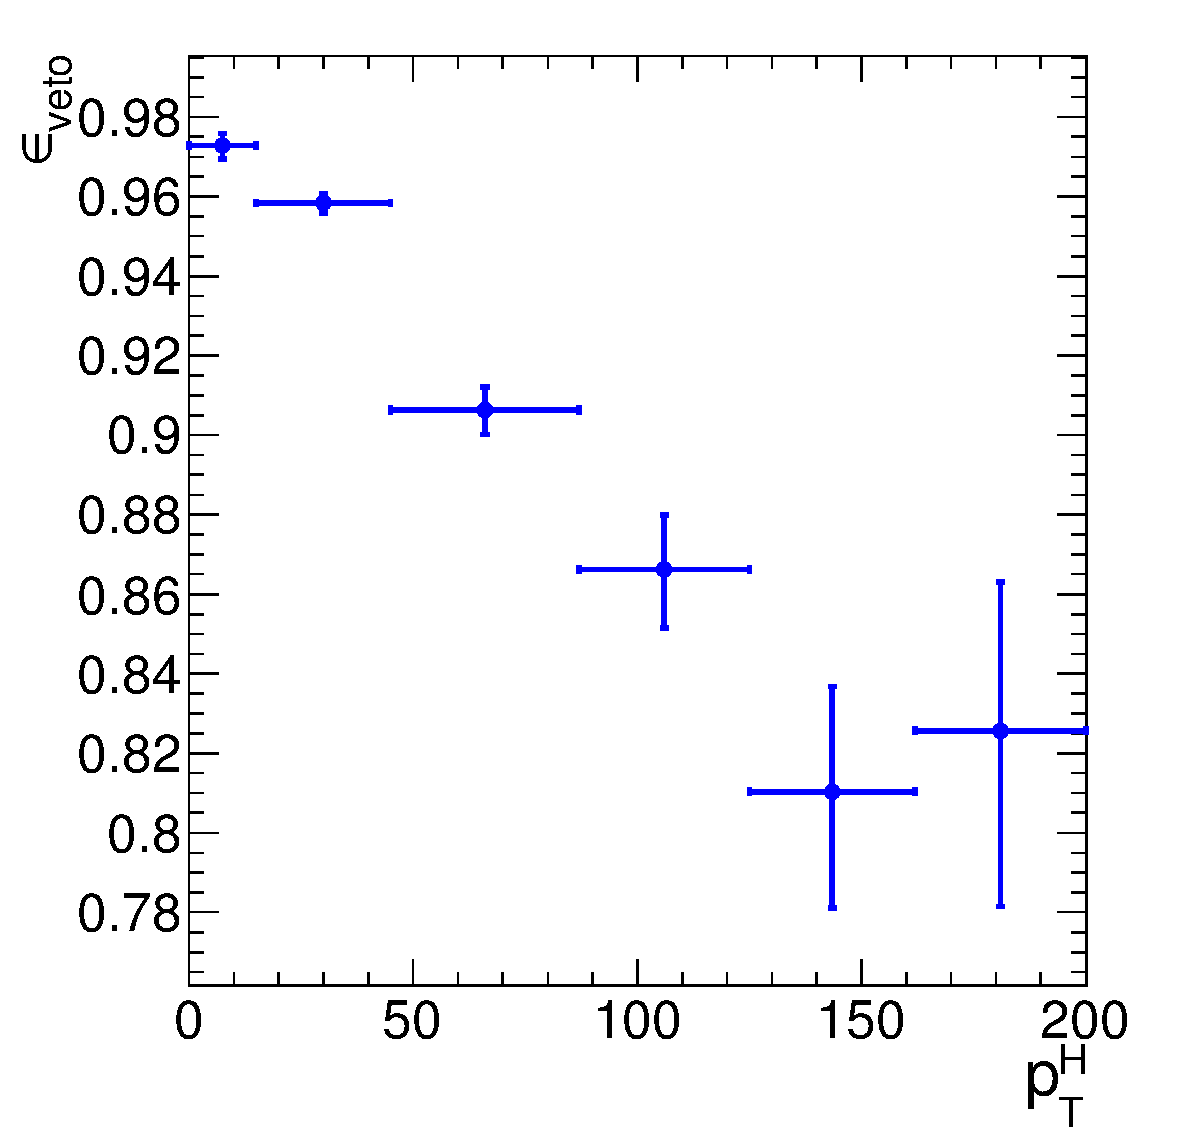
\includegraphics[width=0.45\textwidth]{images/eff_vs_pth.pdf}
		\label{fig:veto_eff_pth}
	}
	\subfigure[]{
		\centering
		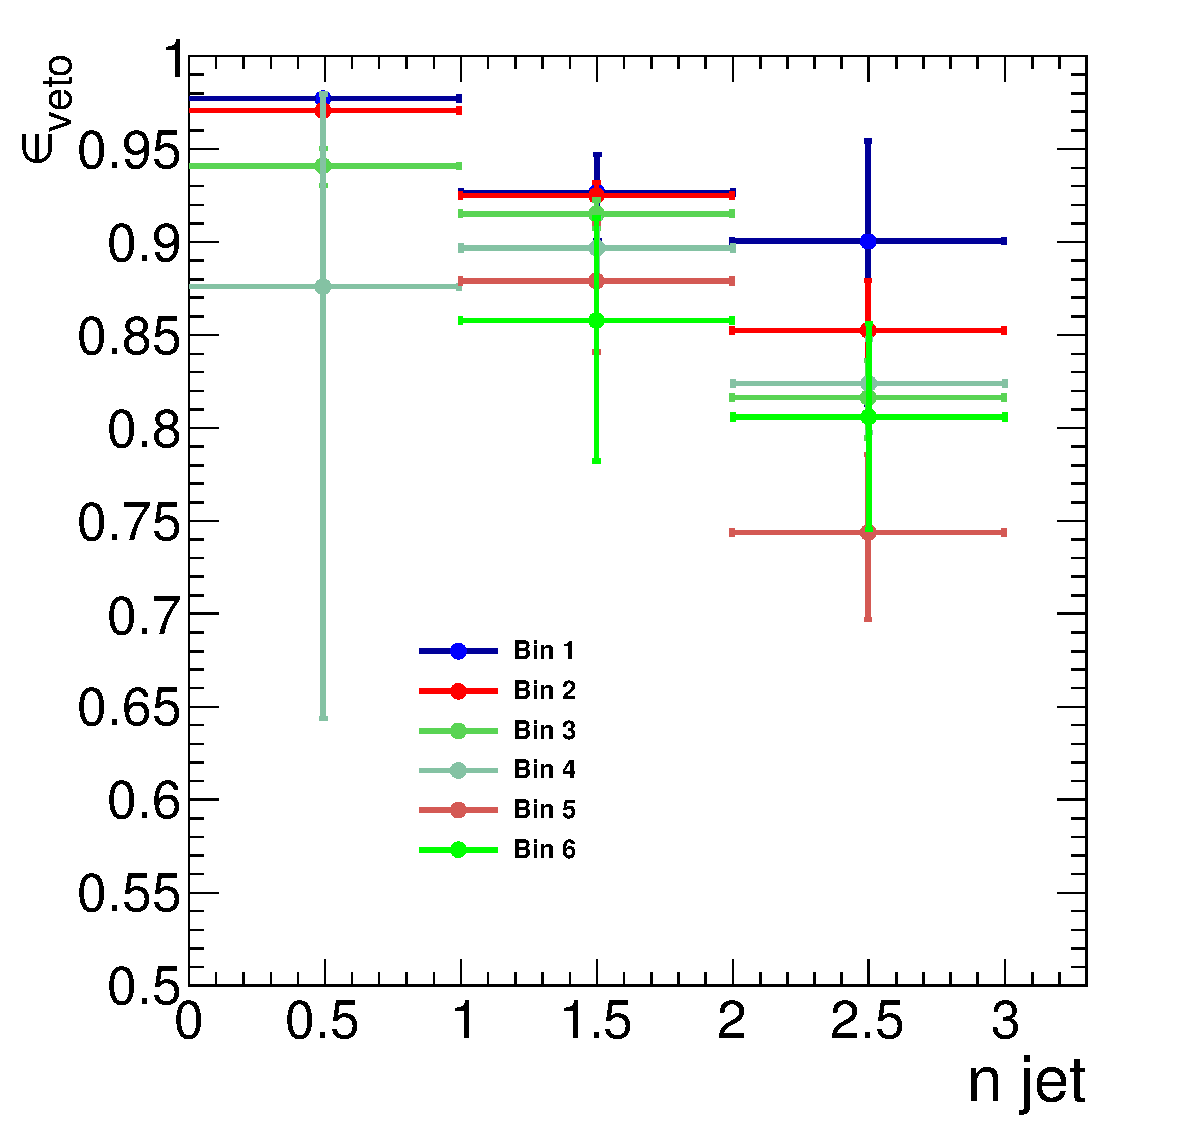
\includegraphics[width=0.45\textwidth]{images/eff_vs_jet.pdf}
		\label{fig:veto_eff_njet}
	}
\caption{(a) Efficiency of the b-tagging veto in different bins of \pth. (b) Efficiency of the b-tagging veto in different bins of \pth, as a function of number of jets.}
\end{figure}

The first step of this procedure is to take the inclusive ggH cross section, $\sigma_\mathrm{ggH}$, and to convert the relative QCD up/down scale uncertainties, $\epsilon_+$ and $\epsilon_-$, to a log-normal uncertainty, i.e. $\kappa = \sqrt{\exp{(\epsilon_+)}\cdot \exp{(\epsilon_-)}}$. The exclusive cross sections, $\sigma_0$, $\sigma_1$ and $\sigma_2$, can be calculated starting from $\sigma_\mathrm{ggH}$ and using the selection efficiencies for the three jet bins. For every exclusive cross section the corresponding relative uncertainty is computed varying the renormalization ($\mu_R$) and factorization ($\mu_F$) scales independently of a factor 2 and $1/2$, and taking the cross section value corresponding to half of the maximum variation. The inclusive cross sections are then obtained summing the exclusive cross sections and propagating the uncertainties, i.e. $\sigma_{\geq 0 } = \sigma_0 + \sigma_1 + \sigma_2$, $\sigma_{\geq 1} = \sigma_1 + \sigma_2$, $\sigma_{\geq 2} = \sigma_2$.

The three nuisance parameters, including all the proper correlations among the jet bins, are defined according to Table~\ref{table:jet_binning_theory}, where the $f_n$ constants represent the exclusive theoretical $n$ jet bin fractions, i.e. $f_0 = \sigma_0/\sigma_{\geq 0}$, $f_1 = \sigma_1/\sigma_{\geq 0}$, $f_2 = \sigma_2/\sigma_{\geq 0}$.

\begin{table}[h]
\caption{Numerical calculation for the systematic uncertainties of jet binning.}
\label{table:jet_binning_theory}
\begin{center}
\begin{tabular}{|l|c|c|c|}
\hline
Nuisance parameter & 0-jet bin                                              & 1-jet bin                                            & 2-jet bin \\ 
\hline
&&& \\
QCDscale\_ggH          & $\Delta^0_{\geq 0} = (\kappa_{\ge 0})^{\frac{1}{f_0}} $    &      & \\ 
&&&\\\hline
&&&\\
QCDscale\_ggH1in       & $\Delta^0_{\geq 1} = (\kappa_{\ge 1})^{- \frac{f_1 + f_2}{f_0}} $ & $\Delta^1_{\geq 1} = (\kappa_{\ge 1})^{\frac{f_1 + f_2}{f_1}} $ & \\ 
&&&\\ \hline
&&&\\
QCDscale\_ggH2in        &                                                        & $\Delta^1_{\geq 2} = (\kappa_{\ge 2})^{- \frac{f_2}{f_1}} $     & $\Delta^2_{\geq 2} = (\kappa_{\ge 2})$ \\ 
&&&\\\hline

\end{tabular}
\end{center}
\end{table}

The nuisance parameters reported in table \ref{table:jet_binning_theory} have then been calculated for each \pth bin embedding the b-jet veto efficiency and using the following formulas:
\begin{equation}
\emph{QCDscale\_ggH}=\frac{\Delta^0_{\geq 0}\cdot f_{0}\cdot \varepsilon_{0}+\Delta^0_{\geq 1}\cdot f_{1}\cdot\varepsilon_{1}}{\Delta^0_{\geq 0}\cdot f_{0}\cdot \varepsilon_{0}+\Delta^0_{\geq 1}\cdot f_{1}\cdot \varepsilon_{0}} \quad,
\end{equation}
\begin{equation}
\emph{QCDscale\_ggH1in}=\frac{\Delta^1_{\geq 1}\cdot f_{1}\cdot \varepsilon_{1}+\Delta^1_{\geq 2}\cdot f_{2}\cdot \varepsilon_{2}}{\Delta^1_{\geq 1}\cdot f_{1} \cdot \varepsilon_{1}+\Delta^1_{\geq 2}\cdot f_{2}\cdot \varepsilon_{1}} \quad,
\end{equation}
\begin{equation}
QCDscale\_ggH2in=1 \quad,
\end{equation}
where $\varepsilon_0$, $\varepsilon_1$ and $\varepsilon_2$ are the selection efficiencies for the three jet categories.
These nuisance parameters are expected to be equal to one in case the efficiency is independent on the number of jets, i.e if $\varepsilon_0 = \varepsilon_1 = \varepsilon_2$.\\
The numerical values obtained following this procedure are reported in Table~\ref{table:jet_binning_meas} for each \pth bin.

\begin{table}[h]
\caption{Values of the jet binning nuisance parameters for different \pth bins.}
\label{table:jet_binning_meas}
\begin{center}
\begin{tabular}{ccccccc}
\toprule
\multirow{2}{*}{Nuisance parameter} & \multicolumn{6}{c}{\pth bin [GeV]} \\
& [0-15] & [15-45] & [45-85] & [85-125] & [125-165] & [165-$\infty$]\\
\midrule
QCDscale\_ggH  & 0.998  &   0.993  &   0.989  &   1.000  &   1.000   &  1.000 \\
QCDscale\_ggH1in &0.997   &  0.993  &   0.984  &   0.975 &    0.946 &    0.974  \\
\bottomrule
\end{tabular}
\end{center}
\end{table}


%-------------------------------------------------------------------------------
\subsection{Statistics uncertainty of the simulated samples}
%-------------------------------------------------------------------------------

Due to the large range of weights used to correct the simulated distributions in order to
match those in data, the effective size of the MC samples are sometimes smaller than
the actual number of events in the sample.
The statistical uncertainties of the event yields estimated from MC samples
are included as nuisance parameters in the fit and have a small impact on the final result.

%-------------------------------------------------------------------------------
\subsection{Treatment of systematic uncertainties in the shape analysis}\label{sec:syst_treatment}
%-------------------------------------------------------------------------------

One can distinguish between normalization uncertainties, where a systematic
effect is changing the normalization of a given process assuming the shape is not affected, and
shape uncertainties where the actual change in the shape of the distribution is
taken into account. The normalization uncertainties enter the shape analysis as
a constant normalization factor, whereas for shape uncertainties the nominal and
the $+1\sigma$ and $-1\sigma$ shapes enter the analysis in form of three histograms
with the same normalization. 

For the W+jets background, the shape differences for different jet \pt thresholds in the 
di-jet control sample are considered separately for electron and muon fakes, while the
other sources of systematics are taken as normalization uncertainties as in the cut-based
analysis.

Effects from experimental uncertainties are studied by applying a scaling and smearing of certain variables of the physics objects, followed by a subsequent
recalculation of all the correlated variables. This is done for simulation, to account for possible systematic mis-measurements of the data.
All experimental sources from Section~\ref{subsec:expsyst} but luminosity
are treated both as normalization and shape uncertainties.
For background with a data-driven normalization estimation,
only the shape uncertainty is considered.

To account for statistical uncertainties, for each distribution going into the shape analysis, 
the $+1\sigma$ and $-1\sigma$ shapes were obtained by adding/subtracting the statistical error 
in each bin and renormalizing it to the nominal distribution. In addition to this procedure a constant 
normalization uncertainty due to the finite statistics of the MC sample used to extract the shape is assigned.

